\documentclass[11pt]{article}
\usepackage{mypackages}
\begin{document}

\maketitle

\section{Data}\label{Data}

To train and test our actor-critic and advantage asynchronous actor-critic implementation we will use
the OpenAI Gym framework\cite{openAIGym}.
This framework provides an interface to 118 Atari 2600 games,
that can be used by developers to compare and test their reinforcement learning algorithms.

 
In the Atari enviroments there is always a finite \textit{action space} and a continous \textit{state space}.
The state space is continous because a \textit{state} is represented as a RGB image - a screenshot - from a game
at the given time and the action space is finite because there is always a fixed amount of
actions available to the player.

Simulating an action in a game return information about the new state,
a \textit{reward} for taking said action and a \textit{binary signal} which indicate whether the 
game is done or not.
The reward is the score the game has registered in the new state.
It is not uncommon for this reward to be $0$ as many of the players actions doesn't produce an immediate reward.

\subsection{Cart-Pole}

OpenAI gym also supports an additional interface we will be using, which is made for the Cart-Pole problem.
A player wins the Cart-Pole game if he manages to balance a pole connected to the top of a moving cart for
200 time steps.
The player loses if the pole moves to more than 15 degrees from vertical
or if the cart exits the frame.

\begin{figure}[!h]
    \centering
    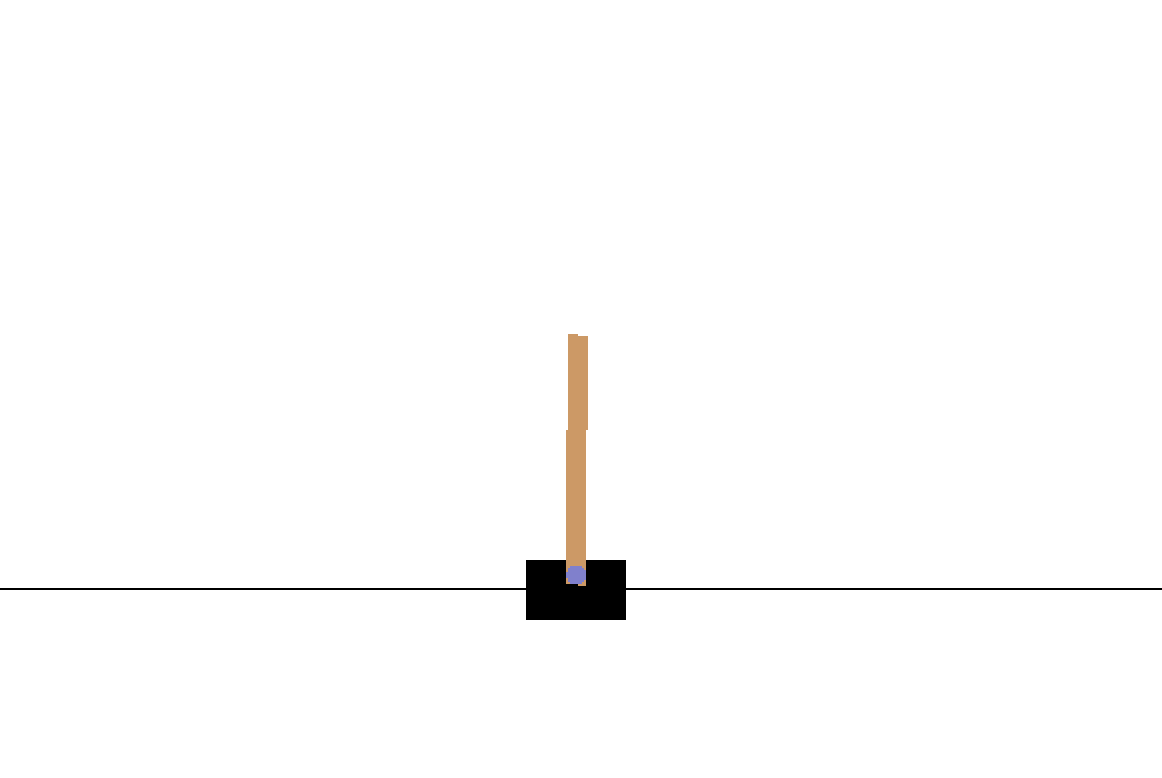
\includegraphics[scale=0.5]{include/cartpole.png}
    \caption{A frame from Cart-Pole.}
    \label{fig:cartpole}
\end{figure}

Unlike the Atari environments a state in Cart-Pole consits of only four elements - the position, and velocity, of the cart and the
angle, and angular velocity, of the pole.
Each time step the player has to chose between moving the cart to the right or to the left and it is not possible
to do nothing.
For every time step the pole doesn't move 15 degrees from vertical the player is awarded a single point.

We will be using the Cart-Pole problem as a proof of concept for our actor-critic implementation and will
compare it to the A3C algorithm used on the same problem.
The reason for this choice is that the problem should be easier to solve, because the
states have fewer dimensions.


\subsection{Atari 2600 games}

As mentioned earlier the interface to Atari games resembles the one focused on the Cart-Pole problem,
with the difference being that we are given the RGB values of a frame from the game
instead of a vector containing information about the environment.
This means that instead of only taking 4 items into consideration when picking an action,
the player is now faced with a 3-dimensional matrix representing a frame.
All of the games have the same resolution of $210 \times 160$ pixels.
Each pixel contains three channels corresponding to the red, green and blue intensities of the pixel.

Using the raw Atari frames can be computationally demanding, so we have chosen
to preprocess our data as described in \cite{dqn}. 
\begin{figure}[!h]
    \centering
    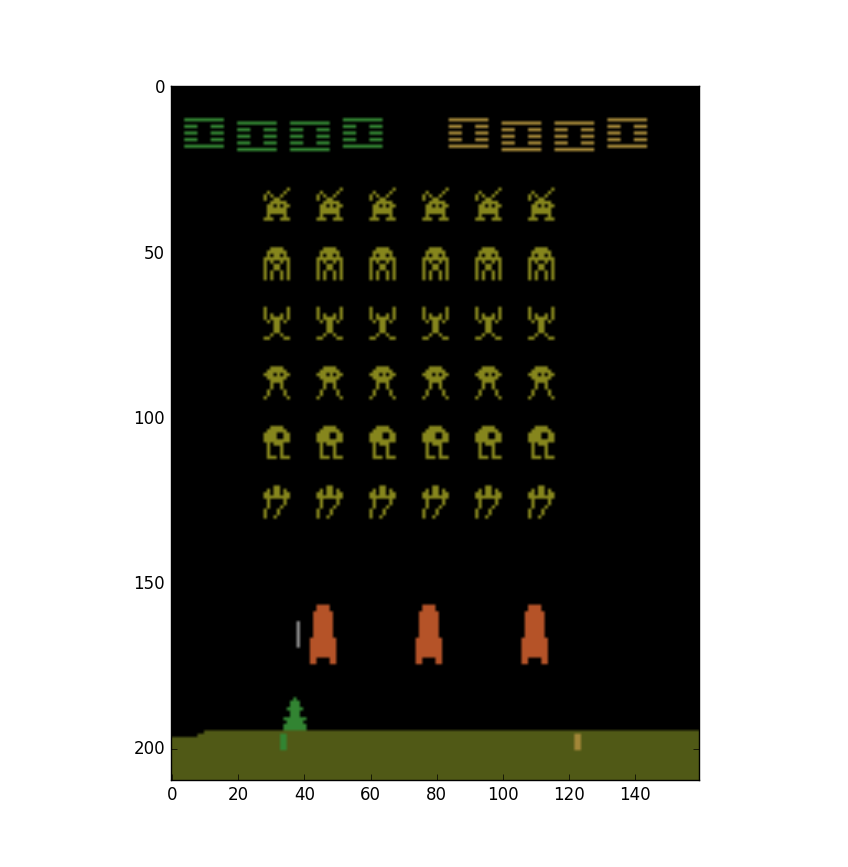
\includegraphics[scale=0.35]{include/space_invaders_1.png}
    \caption{A raw RGB frame from \textit{Space Invaders}.}
    \label{fig:si}
\end{figure}
The first step of the preprocessing is to reduce the amount of channels needed to
represent the image.
To do this we gray-scale the RGB images so that only a single channel is used.
In our approach, the gray-scaling calculates the relative luminance\cite{luminance} of each pixel and the formula is given in equation \ref{eq:lum}.
\begin{equation}\label{eq:lum}
    L(R, G, B) = 0.2126*R + 0.7152*G + 0.0722*B
\end{equation}

\begin{figure}[!h]
    \centering
    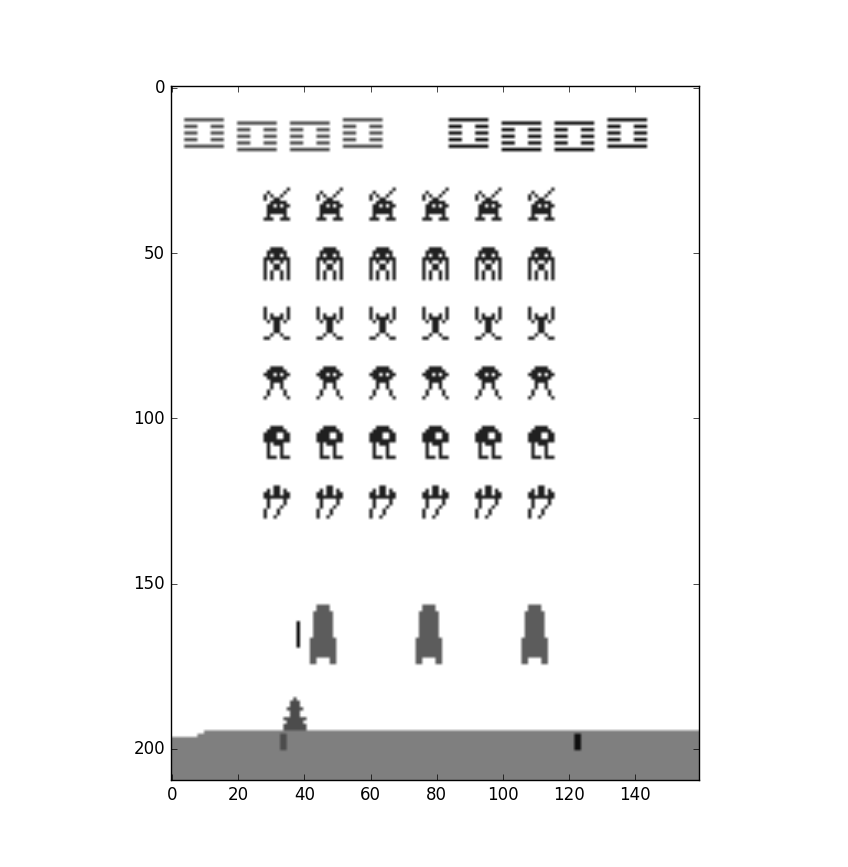
\includegraphics[scale=0.35]{include/space_invaders_1_gray.png}
    \caption{The gray-scaled frame from figure \ref{fig:si}.}
    \label{fig:sig}
\end{figure}

We further reduce the dimensions of the gray-scaled images by a downsampling.
We simply ignore every second pixel effectively halfing the resolution of the images
in both dimensions.

\begin{figure}[!h]
    \centering
    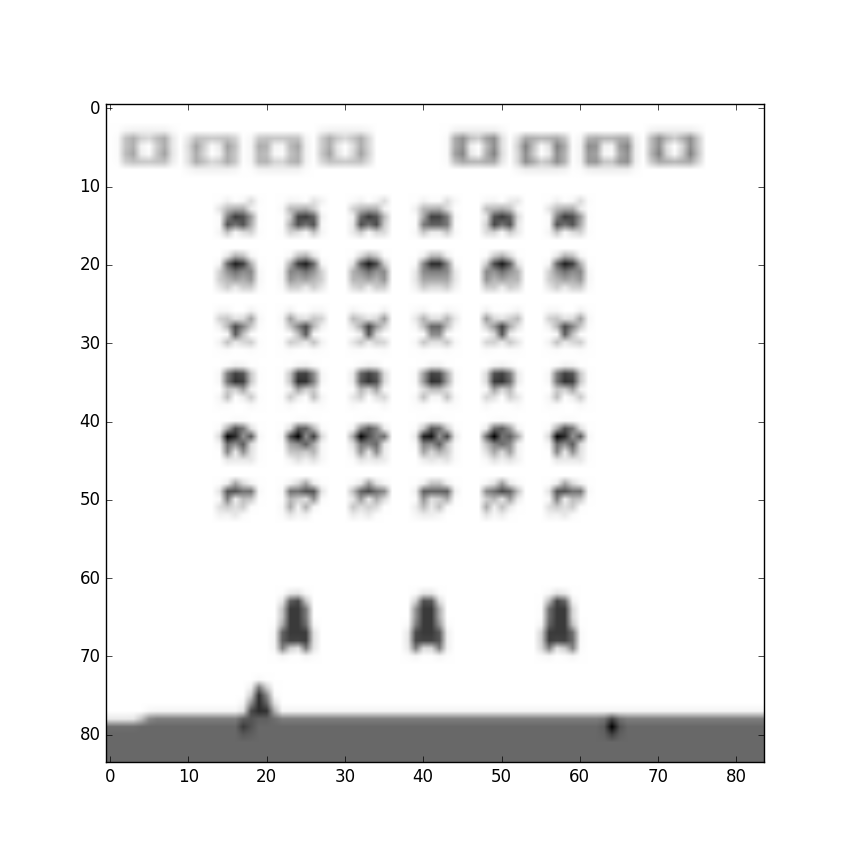
\includegraphics[scale=0.35]{include/space_invaders_1_gray_resized.png}
    \caption{The result of resizing the gray-scaled frame from figure \ref{sig}.}
    \label{fig:sigr}
\end{figure}

Thus, the final output of the preprocessing step is $105 \times 80$ pixel gray-scaled
images.
After the data has been preprocessed it is computationally cheaper to extract the remaining
features than it would be to extract them from the raw Atari frames.
The reason we can reduce the dimensionalities of the frames this way
is due to an assumption about the structure of the data - that
little to no information is lost in the process.



In the articles \cite{a3c} and \cite{dqn} one more preprocessingstep is performed.
Instead of only resizing the grey-scaled frames, they are also cropped to $84 \times 84$ images.
This is done to meet a condition in their implementation of 2d convolutions,
since they could only process square input\cite{dqn-nature}.
We will only be resizing the gray-scaled images and not be cropping,
since the cropping doesn't serve the same purpose in our project.
Another consideration about cropping the images is it is difficult to assume that no
information is lost when a large chunk of the data is removed.
This project aims at a generalized solution that is able to learn to play any Atari game.
If the images were to be cropped in the same manner,
the different structure of the frames of each game would lead to an unstable
result, meaning we would have to handcraft a cropping scheme for each game.

Due to the time limitations of this project we will only be testing our
implementation of the A3C algorithm on certain games.
Namely \textit{Pong}, \textit{Breakout}, \textit{Space Invaders} and
\textit{Pacman}.

\end{document}
